\documentclass[class=minimal,border=0pt]{standalone}
\usepackage{hyperref}
\hypersetup{
colorlinks=true,
urlcolor=cyan}
\usepackage{tikz}
\begin{document}
%\documentclass{standalone}
%\usepackage{tikz}
%\usetikzlibrary{patterns,plotmarks}
%\begin{document}
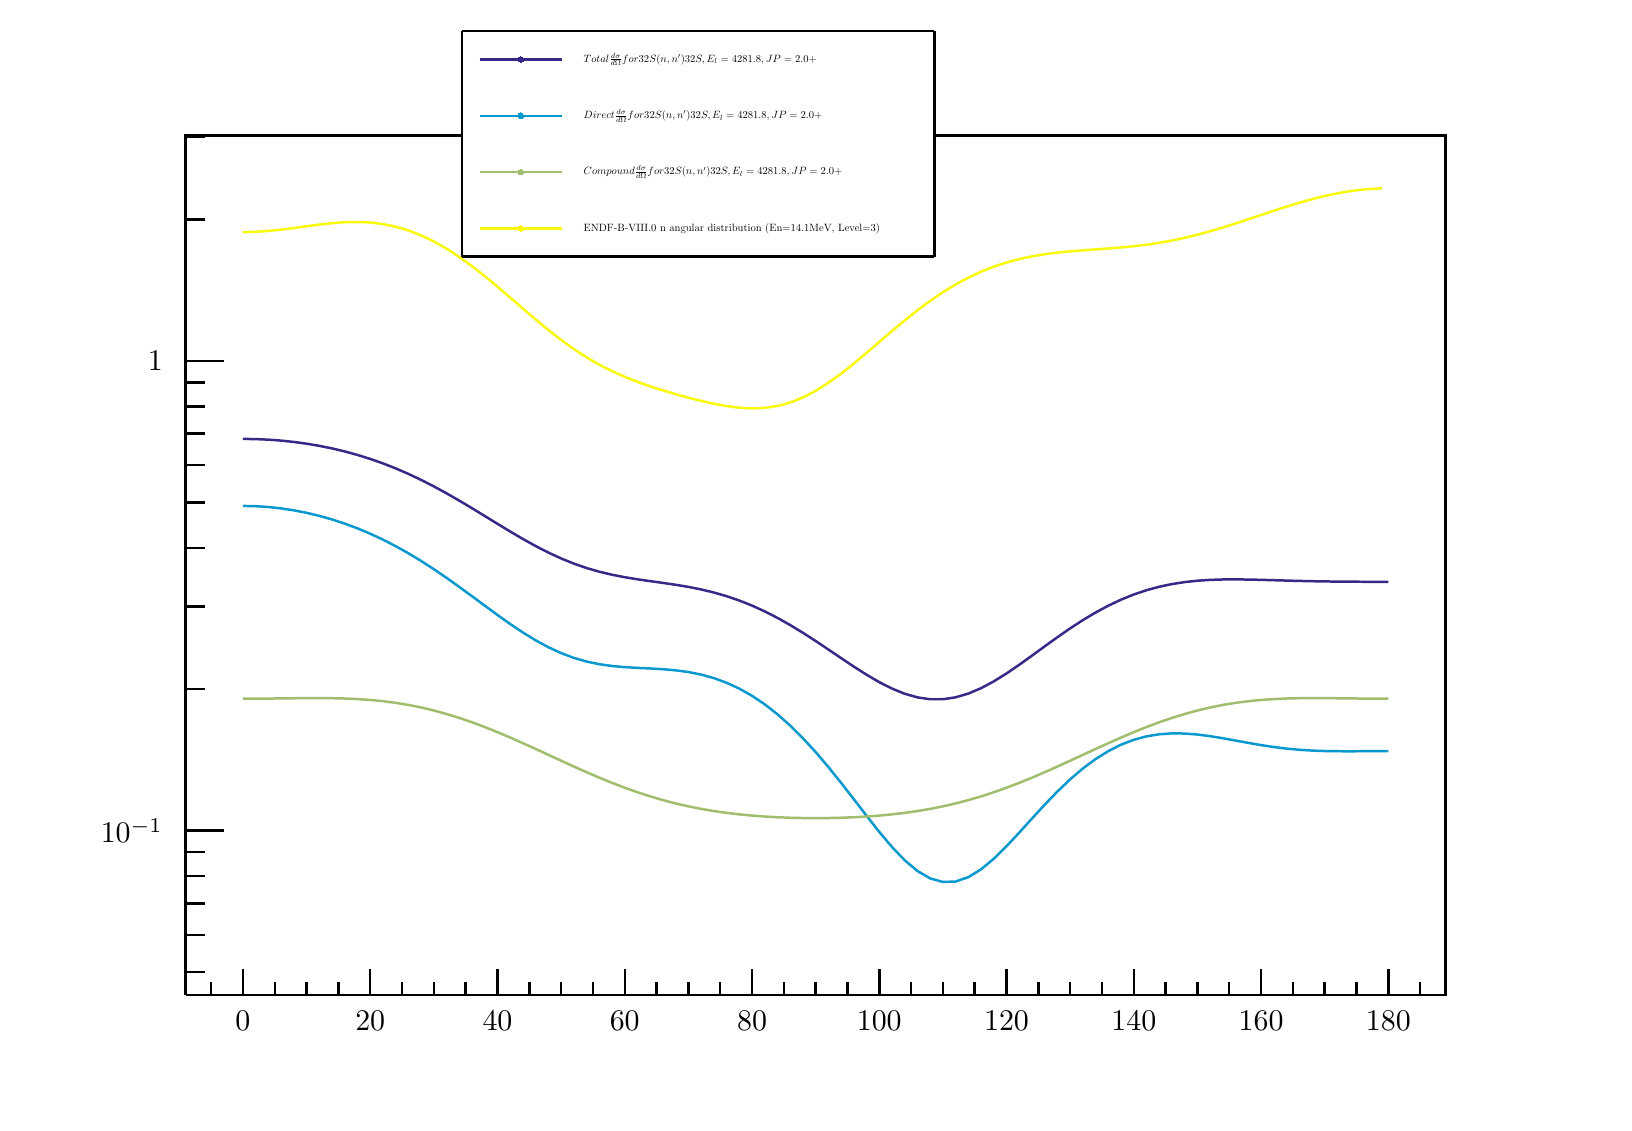
\begin{tikzpicture}
\def\CheckTikzLibraryLoaded#1{ \ifcsname tikz@library@#1@loaded\endcsname \else \PackageWarning{tikz}{usetikzlibrary{#1} is missing in the preamble.} \fi }
\CheckTikzLibraryLoaded{patterns}
\CheckTikzLibraryLoaded{plotmarks}
\pgfdeclareplotmark{cross} {
\pgfpathmoveto{\pgfpoint{-0.3\pgfplotmarksize}{\pgfplotmarksize}}
\pgfpathlineto{\pgfpoint{+0.3\pgfplotmarksize}{\pgfplotmarksize}}
\pgfpathlineto{\pgfpoint{+0.3\pgfplotmarksize}{0.3\pgfplotmarksize}}
\pgfpathlineto{\pgfpoint{+1\pgfplotmarksize}{0.3\pgfplotmarksize}}
\pgfpathlineto{\pgfpoint{+1\pgfplotmarksize}{-0.3\pgfplotmarksize}}
\pgfpathlineto{\pgfpoint{+0.3\pgfplotmarksize}{-0.3\pgfplotmarksize}}
\pgfpathlineto{\pgfpoint{+0.3\pgfplotmarksize}{-1.\pgfplotmarksize}}
\pgfpathlineto{\pgfpoint{-0.3\pgfplotmarksize}{-1.\pgfplotmarksize}}
\pgfpathlineto{\pgfpoint{-0.3\pgfplotmarksize}{-0.3\pgfplotmarksize}}
\pgfpathlineto{\pgfpoint{-1.\pgfplotmarksize}{-0.3\pgfplotmarksize}}
\pgfpathlineto{\pgfpoint{-1.\pgfplotmarksize}{0.3\pgfplotmarksize}}
\pgfpathlineto{\pgfpoint{-0.3\pgfplotmarksize}{0.3\pgfplotmarksize}}
\pgfpathclose
\pgfusepathqstroke
}
\pgfdeclareplotmark{cross*} {
\pgfpathmoveto{\pgfpoint{-0.3\pgfplotmarksize}{\pgfplotmarksize}}
\pgfpathlineto{\pgfpoint{+0.3\pgfplotmarksize}{\pgfplotmarksize}}
\pgfpathlineto{\pgfpoint{+0.3\pgfplotmarksize}{0.3\pgfplotmarksize}}
\pgfpathlineto{\pgfpoint{+1\pgfplotmarksize}{0.3\pgfplotmarksize}}
\pgfpathlineto{\pgfpoint{+1\pgfplotmarksize}{-0.3\pgfplotmarksize}}
\pgfpathlineto{\pgfpoint{+0.3\pgfplotmarksize}{-0.3\pgfplotmarksize}}
\pgfpathlineto{\pgfpoint{+0.3\pgfplotmarksize}{-1.\pgfplotmarksize}}
\pgfpathlineto{\pgfpoint{-0.3\pgfplotmarksize}{-1.\pgfplotmarksize}}
\pgfpathlineto{\pgfpoint{-0.3\pgfplotmarksize}{-0.3\pgfplotmarksize}}
\pgfpathlineto{\pgfpoint{-1.\pgfplotmarksize}{-0.3\pgfplotmarksize}}
\pgfpathlineto{\pgfpoint{-1.\pgfplotmarksize}{0.3\pgfplotmarksize}}
\pgfpathlineto{\pgfpoint{-0.3\pgfplotmarksize}{0.3\pgfplotmarksize}}
\pgfpathclose
\pgfusepathqfillstroke
}
\pgfdeclareplotmark{newstar} {
\pgfpathmoveto{\pgfqpoint{0pt}{\pgfplotmarksize}}
\pgfpathlineto{\pgfqpointpolar{44}{0.5\pgfplotmarksize}}
\pgfpathlineto{\pgfqpointpolar{18}{\pgfplotmarksize}}
\pgfpathlineto{\pgfqpointpolar{-20}{0.5\pgfplotmarksize}}
\pgfpathlineto{\pgfqpointpolar{-54}{\pgfplotmarksize}}
\pgfpathlineto{\pgfqpointpolar{-90}{0.5\pgfplotmarksize}}
\pgfpathlineto{\pgfqpointpolar{234}{\pgfplotmarksize}}
\pgfpathlineto{\pgfqpointpolar{198}{0.5\pgfplotmarksize}}
\pgfpathlineto{\pgfqpointpolar{162}{\pgfplotmarksize}}
\pgfpathlineto{\pgfqpointpolar{134}{0.5\pgfplotmarksize}}
\pgfpathclose
\pgfusepathqstroke
}
\pgfdeclareplotmark{newstar*} {
\pgfpathmoveto{\pgfqpoint{0pt}{\pgfplotmarksize}}
\pgfpathlineto{\pgfqpointpolar{44}{0.5\pgfplotmarksize}}
\pgfpathlineto{\pgfqpointpolar{18}{\pgfplotmarksize}}
\pgfpathlineto{\pgfqpointpolar{-20}{0.5\pgfplotmarksize}}
\pgfpathlineto{\pgfqpointpolar{-54}{\pgfplotmarksize}}
\pgfpathlineto{\pgfqpointpolar{-90}{0.5\pgfplotmarksize}}
\pgfpathlineto{\pgfqpointpolar{234}{\pgfplotmarksize}}
\pgfpathlineto{\pgfqpointpolar{198}{0.5\pgfplotmarksize}}
\pgfpathlineto{\pgfqpointpolar{162}{\pgfplotmarksize}}
\pgfpathlineto{\pgfqpointpolar{134}{0.5\pgfplotmarksize}}
\pgfpathclose
\pgfusepathqfillstroke
}
\definecolor{c}{rgb}{1,1,1};
\draw [color=c, fill=c] (0,0) rectangle (20,13.639);
\draw [color=c, fill=c] (2,1.3639) rectangle (18,12.2751);
\definecolor{c}{rgb}{0,0,0};
\draw [c,line width=0.9] (2,1.3639) -- (2,12.2751) -- (18,12.2751) -- (18,1.3639) -- (2,1.3639);
\draw [c,line width=0.9] (2,1.3639) -- (18,1.3639);
\draw [c,line width=0.9] (2.72727,1.69123) -- (2.72727,1.3639);
\draw [c,line width=0.9] (3.13131,1.52756) -- (3.13131,1.3639);
\draw [c,line width=0.9] (3.53535,1.52756) -- (3.53535,1.3639);
\draw [c,line width=0.9] (3.93939,1.52756) -- (3.93939,1.3639);
\draw [c,line width=0.9] (4.34343,1.69123) -- (4.34343,1.3639);
\draw [c,line width=0.9] (4.74747,1.52756) -- (4.74747,1.3639);
\draw [c,line width=0.9] (5.15152,1.52756) -- (5.15152,1.3639);
\draw [c,line width=0.9] (5.55556,1.52756) -- (5.55556,1.3639);
\draw [c,line width=0.9] (5.9596,1.69123) -- (5.9596,1.3639);
\draw [c,line width=0.9] (6.36364,1.52756) -- (6.36364,1.3639);
\draw [c,line width=0.9] (6.76768,1.52756) -- (6.76768,1.3639);
\draw [c,line width=0.9] (7.17172,1.52756) -- (7.17172,1.3639);
\draw [c,line width=0.9] (7.57576,1.69123) -- (7.57576,1.3639);
\draw [c,line width=0.9] (7.9798,1.52756) -- (7.9798,1.3639);
\draw [c,line width=0.9] (8.38384,1.52756) -- (8.38384,1.3639);
\draw [c,line width=0.9] (8.78788,1.52756) -- (8.78788,1.3639);
\draw [c,line width=0.9] (9.19192,1.69123) -- (9.19192,1.3639);
\draw [c,line width=0.9] (9.59596,1.52756) -- (9.59596,1.3639);
\draw [c,line width=0.9] (10,1.52756) -- (10,1.3639);
\draw [c,line width=0.9] (10.404,1.52756) -- (10.404,1.3639);
\draw [c,line width=0.9] (10.8081,1.69123) -- (10.8081,1.3639);
\draw [c,line width=0.9] (11.2121,1.52756) -- (11.2121,1.3639);
\draw [c,line width=0.9] (11.6162,1.52756) -- (11.6162,1.3639);
\draw [c,line width=0.9] (12.0202,1.52756) -- (12.0202,1.3639);
\draw [c,line width=0.9] (12.4242,1.69123) -- (12.4242,1.3639);
\draw [c,line width=0.9] (12.8283,1.52756) -- (12.8283,1.3639);
\draw [c,line width=0.9] (13.2323,1.52756) -- (13.2323,1.3639);
\draw [c,line width=0.9] (13.6364,1.52756) -- (13.6364,1.3639);
\draw [c,line width=0.9] (14.0404,1.69123) -- (14.0404,1.3639);
\draw [c,line width=0.9] (14.4444,1.52756) -- (14.4444,1.3639);
\draw [c,line width=0.9] (14.8485,1.52756) -- (14.8485,1.3639);
\draw [c,line width=0.9] (15.2525,1.52756) -- (15.2525,1.3639);
\draw [c,line width=0.9] (15.6566,1.69123) -- (15.6566,1.3639);
\draw [c,line width=0.9] (16.0606,1.52756) -- (16.0606,1.3639);
\draw [c,line width=0.9] (16.4646,1.52756) -- (16.4646,1.3639);
\draw [c,line width=0.9] (16.8687,1.52756) -- (16.8687,1.3639);
\draw [c,line width=0.9] (17.2727,1.69123) -- (17.2727,1.3639);
\draw [c,line width=0.9] (2.72727,1.69123) -- (2.72727,1.3639);
\draw [c,line width=0.9] (2.32323,1.52756) -- (2.32323,1.3639);
\draw [c,line width=0.9] (17.2727,1.69123) -- (17.2727,1.3639);
\draw [c,line width=0.9] (17.6768,1.52756) -- (17.6768,1.3639);
\draw [anchor=base] (2.72727,0.913811) node[scale=1.08185, color=c, rotate=0]{0};
\draw [anchor=base] (4.34343,0.913811) node[scale=1.08185, color=c, rotate=0]{20};
\draw [anchor=base] (5.9596,0.913811) node[scale=1.08185, color=c, rotate=0]{40};
\draw [anchor=base] (7.57576,0.913811) node[scale=1.08185, color=c, rotate=0]{60};
\draw [anchor=base] (9.19192,0.913811) node[scale=1.08185, color=c, rotate=0]{80};
\draw [anchor=base] (10.8081,0.913811) node[scale=1.08185, color=c, rotate=0]{100};
\draw [anchor=base] (12.4242,0.913811) node[scale=1.08185, color=c, rotate=0]{120};
\draw [anchor=base] (14.0404,0.913811) node[scale=1.08185, color=c, rotate=0]{140};
\draw [anchor=base] (15.6566,0.913811) node[scale=1.08185, color=c, rotate=0]{160};
\draw [anchor=base] (17.2727,0.913811) node[scale=1.08185, color=c, rotate=0]{180};
\draw [c,line width=0.9] (2,1.3639) -- (2,12.2751);
\draw [c,line width=0.9] (2.24,1.6516) -- (2,1.6516);
\draw [c,line width=0.9] (2.24,2.12407) -- (2,2.12407);
\draw [c,line width=0.9] (2.24,2.52354) -- (2,2.52354);
\draw [c,line width=0.9] (2.24,2.86958) -- (2,2.86958);
\draw [c,line width=0.9] (2.24,3.1748) -- (2,3.1748);
\draw [c,line width=0.9] (2.48,3.44784) -- (2,3.44784);
\draw [anchor= east] (1.844,3.44784) node[scale=1.08185, color=c, rotate=0]{$10^{-1}$};
\draw [c,line width=0.9] (2.24,5.24408) -- (2,5.24408);
\draw [c,line width=0.9] (2.24,6.29481) -- (2,6.29481);
\draw [c,line width=0.9] (2.24,7.04032) -- (2,7.04032);
\draw [c,line width=0.9] (2.24,7.61858) -- (2,7.61858);
\draw [c,line width=0.9] (2.24,8.09105) -- (2,8.09105);
\draw [c,line width=0.9] (2.24,8.49052) -- (2,8.49052);
\draw [c,line width=0.9] (2.24,8.83656) -- (2,8.83656);
\draw [c,line width=0.9] (2.24,9.14179) -- (2,9.14179);
\draw [c,line width=0.9] (2.48,9.41482) -- (2,9.41482);
\draw [anchor= east] (1.844,9.41482) node[scale=1.08185, color=c, rotate=0]{1};
\draw [c,line width=0.9] (2.24,11.2111) -- (2,11.2111);
\draw [c,line width=0.9] (2.24,12.2618) -- (2,12.2618);
\definecolor{c}{rgb}{0.2082,0.1664,0.5293};
\draw [c,line width=0.9] (2.72727,8.42323) -- (2.88889,8.42083) -- (3.05051,8.41363) -- (3.21212,8.40157) -- (3.37374,8.38456) -- (3.53535,8.36249) -- (3.69697,8.33518) -- (3.85859,8.30244) -- (4.0202,8.26402) -- (4.18182,8.21969) --
 (4.34343,8.16918) -- (4.50505,8.11229) -- (4.66667,8.04888) -- (4.82828,7.97891) -- (4.9899,7.9025) -- (5.15152,7.81998) -- (5.31313,7.7319) -- (5.47475,7.6391) -- (5.63636,7.54269) -- (5.79798,7.44405) -- (5.9596,7.34485) -- (6.12121,7.2469) --
 (6.28283,7.15216) -- (6.44444,7.0625) -- (6.60606,6.97965) -- (6.76768,6.90501) -- (6.92929,6.8395) -- (7.09091,6.78349) -- (7.25253,6.73667) -- (7.41414,6.6982) -- (7.57576,6.66668) -- (7.73737,6.64029) -- (7.89899,6.61696) -- (8.06061,6.59449) --
 (8.22222,6.57075) -- (8.38384,6.54369) -- (8.54545,6.51153) -- (8.70707,6.47275) -- (8.86869,6.42617) -- (9.0303,6.37093) -- (9.19192,6.30655) -- (9.35354,6.2329) -- (9.51515,6.15025) -- (9.67677,6.05922) -- (9.83838,5.9609) -- (10,5.85677) --
 (10.1616,5.74881) -- (10.3232,5.63945) -- (10.4848,5.53162) -- (10.6465,5.42869) -- (10.8081,5.33433) -- (10.9697,5.25242) -- (11.1313,5.18675) -- (11.2929,5.1407) -- (11.4545,5.11693) -- (11.6162,5.11704) -- (11.7778,5.14139) -- (11.9394,5.189) --
 (12.101,5.25762) -- (12.2626,5.34408) -- (12.4242,5.44452) -- (12.5859,5.55481) -- (12.7475,5.67082) -- (12.9091,5.78871) -- (13.0707,5.90506) -- (13.2323,6.01698) -- (13.3939,6.12214) -- (13.5556,6.21877) -- (13.7172,6.30561) -- (13.8788,6.38187)
 -- (14.0404,6.44723) -- (14.202,6.50171) -- (14.3636,6.54568) -- (14.5253,6.57979) -- (14.6869,6.60495) -- (14.8485,6.62222) -- (15.0101,6.63281) -- (15.1717,6.63798) -- (15.3333,6.63901) -- (15.4949,6.63711) -- (15.6566,6.63339) --
 (15.8182,6.62878) -- (15.9798,6.62402) -- (16.1414,6.61965) -- (16.303,6.61597) -- (16.4646,6.61314) -- (16.6263,6.61111) -- (16.7879,6.6098) -- (16.9495,6.60903) -- (17.1111,6.60863) -- (17.2727,6.60851);
\definecolor{c}{rgb}{0.040325,0.598837,0.806119};
\draw [c,line width=0.9] (2.72727,7.57214) -- (2.88889,7.56863) -- (3.05051,7.55811) -- (3.21212,7.54059) -- (3.37374,7.51605) -- (3.53535,7.4845) -- (3.69697,7.4459) -- (3.85859,7.40018) -- (4.0202,7.34725) -- (4.18182,7.28698) -- (4.34343,7.21926)
 -- (4.50505,7.14397) -- (4.66667,7.06109) -- (4.82828,6.9707) -- (4.9899,6.87307) -- (5.15152,6.76869) -- (5.31313,6.65839) -- (5.47475,6.54333) -- (5.63636,6.42508) -- (5.79798,6.30562) -- (5.9596,6.18728) -- (6.12121,6.07264) -- (6.28283,5.96446)
 -- (6.44444,5.86536) -- (6.60606,5.77765) -- (6.76768,5.70304) -- (6.92929,5.64243) -- (7.09091,5.59577) -- (7.25253,5.562) -- (7.41414,5.53918) -- (7.57576,5.52465) -- (7.73737,5.51526) -- (7.89899,5.50763) -- (8.06061,5.49837) -- (8.22222,5.48427)
 -- (8.38384,5.46241) -- (8.54545,5.43025) -- (8.70707,5.38558) -- (8.86869,5.32668) -- (9.0303,5.25214) -- (9.19192,5.16094) -- (9.35354,5.05244) -- (9.51515,4.92637) -- (9.67677,4.78284) -- (9.83838,4.62244) -- (10,4.44635) -- (10.1616,4.25643) --
 (10.3232,4.05549) -- (10.4848,3.8474) -- (10.6465,3.63751) -- (10.8081,3.43256) -- (10.9697,3.24092) -- (11.1313,3.07211) -- (11.2929,2.9361) -- (11.4545,2.84197) -- (11.6162,2.7964) -- (11.7778,2.80222) -- (11.9394,2.85774) -- (12.101,2.9571) --
 (12.2626,3.0914) -- (12.4242,3.25034) -- (12.5859,3.42367) -- (12.7475,3.60213) -- (12.9091,3.77805) -- (13.0707,3.94541) -- (13.2323,4.09971) -- (13.3939,4.23785) -- (13.5556,4.35785) -- (13.7172,4.45863) -- (13.8788,4.53986) -- (14.0404,4.60188)
 -- (14.202,4.64554) -- (14.3636,4.67214) -- (14.5253,4.68346) -- (14.6869,4.68157) -- (14.8485,4.66886) -- (15.0101,4.64794) -- (15.1717,4.6215) -- (15.3333,4.5922) -- (15.4949,4.56254) -- (15.6566,4.53465) -- (15.8182,4.51019) -- (15.9798,4.49023)
 -- (16.1414,4.47526) -- (16.303,4.46513) -- (16.4646,4.45926) -- (16.6263,4.45666) -- (16.7879,4.45623) -- (16.9495,4.45686) -- (17.1111,4.45763) -- (17.2727,4.45796);
\definecolor{c}{rgb}{0.629272,0.743563,0.426222};
\draw [c,line width=0.9] (2.72727,5.12391) -- (2.88889,5.12438) -- (3.05051,5.12568) -- (3.21212,5.12754) -- (3.37374,5.12953) -- (3.53535,5.13111) -- (3.69697,5.1316) -- (3.85859,5.13027) -- (4.0202,5.12638) -- (4.18182,5.11919) -- (4.34343,5.108)
 -- (4.50505,5.09218) -- (4.66667,5.07123) -- (4.82828,5.04472) -- (4.9899,5.01239) -- (5.15152,4.97411) -- (5.31313,4.9299) -- (5.47475,4.87992) -- (5.63636,4.82449) -- (5.79798,4.76404) -- (5.9596,4.69919) -- (6.12121,4.63061) -- (6.28283,4.55913)
 -- (6.44444,4.48563) -- (6.60606,4.41105) -- (6.76768,4.33637) -- (6.92929,4.26253) -- (7.09091,4.1905) -- (7.25253,4.12109) -- (7.41414,4.0551) -- (7.57576,3.99317) -- (7.73737,3.93579) -- (7.89899,3.88333) -- (8.06061,3.83598) -- (8.22222,3.79381)
 -- (8.38384,3.75674) -- (8.54545,3.72459) -- (8.70707,3.69713) -- (8.86869,3.67403) -- (9.0303,3.65494) -- (9.19192,3.63949) -- (9.35354,3.62738) -- (9.51515,3.61829) -- (9.67677,3.61198) -- (9.83838,3.60828) -- (10,3.60703) -- (10.1616,3.60828) --
 (10.3232,3.61198) -- (10.4848,3.61829) -- (10.6465,3.62738) -- (10.8081,3.63949) -- (10.9697,3.65494) -- (11.1313,3.67403) -- (11.2929,3.69713) -- (11.4545,3.72459) -- (11.6162,3.75674) -- (11.7778,3.79381) -- (11.9394,3.83598) -- (12.101,3.88333)
 -- (12.2626,3.93579) -- (12.4242,3.99317) -- (12.5859,4.0551) -- (12.7475,4.12109) -- (12.9091,4.1905) -- (13.0707,4.26253) -- (13.2323,4.33637) -- (13.3939,4.41105) -- (13.5556,4.48563) -- (13.7172,4.55913) -- (13.8788,4.63061) -- (14.0404,4.69919)
 -- (14.202,4.76404) -- (14.3636,4.82449) -- (14.5253,4.87992) -- (14.6869,4.9299) -- (14.8485,4.97411) -- (15.0101,5.01239) -- (15.1717,5.04472) -- (15.3333,5.07123) -- (15.4949,5.09218) -- (15.6566,5.108) -- (15.8182,5.11919) -- (15.9798,5.12638)
 -- (16.1414,5.13027) -- (16.303,5.1316) -- (16.4646,5.13111) -- (16.6263,5.12953) -- (16.7879,5.12754) -- (16.9495,5.12568) -- (17.1111,5.12438) -- (17.2727,5.12391);
\definecolor{c}{rgb}{0.977,0.977044,0.0583656};
\draw [c,line width=0.9] (2.72727,11.0501) -- (2.80808,11.051) -- (2.88889,11.0538) -- (2.9697,11.0583) -- (3.05051,11.0645) -- (3.13131,11.0721) -- (3.21212,11.0809) -- (3.29293,11.0908) -- (3.37374,11.1014) -- (3.45455,11.1124) -- (3.53535,11.1236)
 -- (3.61616,11.1345) -- (3.69697,11.145) -- (3.77778,11.1545) -- (3.85859,11.1628) -- (3.93939,11.1696) -- (4.0202,11.1745) -- (4.10101,11.1774) -- (4.18182,11.1778) -- (4.26263,11.1756) -- (4.34343,11.1705) -- (4.42424,11.1623) -- (4.50505,11.1509)
 -- (4.58586,11.136) -- (4.66667,11.1177) -- (4.74747,11.0957) -- (4.82828,11.07) -- (4.90909,11.0406) -- (4.9899,11.0074) -- (5.07071,10.9706) -- (5.15152,10.9301) -- (5.23232,10.886) -- (5.31313,10.8384) -- (5.39394,10.7875) -- (5.47475,10.7334) --
 (5.55556,10.6764) -- (5.63636,10.6167) -- (5.71717,10.5545) -- (5.79798,10.4902) -- (5.87879,10.424) -- (5.9596,10.3564) -- (6.0404,10.2876) -- (6.12121,10.218) -- (6.20202,10.1481) -- (6.28283,10.0782) -- (6.36364,10.0088) -- (6.44444,9.94023) --
 (6.52525,9.87285) -- (6.60606,9.80703) -- (6.68687,9.74311) -- (6.76768,9.68137) -- (6.84848,9.62205) -- (6.92929,9.56536) -- (7.0101,9.51143) -- (7.09091,9.46035) -- (7.17172,9.41216) -- (7.25253,9.36684) -- (7.33333,9.32431) -- (7.41414,9.28446)
 -- (7.49495,9.24712) -- (7.57576,9.21213) -- (7.65657,9.17926) -- (7.73737,9.1483) -- (7.81818,9.11904) -- (7.89899,9.09127) -- (7.9798,9.06478) -- (8.06061,9.03941) -- (8.14141,9.01503) -- (8.22222,8.99155) -- (8.30303,8.96891) -- (8.38384,8.94711)
 -- (8.46465,8.92622) -- (8.54545,8.90632) -- (8.62626,8.88759) -- (8.70707,8.87023) -- (8.78788,8.8545) -- (8.86869,8.84071) -- (8.9495,8.82917) -- (9.0303,8.82027) -- (9.11111,8.81437) -- (9.19192,8.81186) -- (9.27273,8.81312) -- (9.35354,8.81848)
 -- (9.43434,8.82827) -- (9.51515,8.84275) -- (9.59596,8.86213) -- (9.67677,8.88654) -- (9.75758,8.91603) -- (9.83838,8.95058) -- (9.91919,8.99008) -- (10,9.03434) -- (10.0808,9.08309) -- (10.1616,9.136) -- (10.2424,9.19267) -- (10.3232,9.25266) --
 (10.404,9.3155) -- (10.4848,9.38069) -- (10.5657,9.44771) -- (10.6465,9.51608) -- (10.7273,9.58527) -- (10.8081,9.65481) -- (10.8889,9.72425) -- (10.9697,9.79316) -- (11.0505,9.86113) -- (11.1313,9.92782) -- (11.2121,9.9929) -- (11.2929,10.0561) --
 (11.3737,10.1171) -- (11.4545,10.1758) -- (11.5354,10.232) -- (11.6162,10.2855) -- (11.697,10.3362) -- (11.7778,10.3841) -- (11.8586,10.4291) -- (11.9394,10.4711) -- (12.0202,10.5102) -- (12.101,10.5465) -- (12.1818,10.5798) -- (12.2626,10.6104) --
 (12.3434,10.6383) -- (12.4242,10.6636) -- (12.5051,10.6863) -- (12.5859,10.7068) -- (12.6667,10.725) -- (12.7475,10.7412) -- (12.8283,10.7555) -- (12.9091,10.7681) -- (12.9899,10.7791) -- (13.0707,10.7888) -- (13.1515,10.7974) -- (13.2323,10.805) --
 (13.3131,10.8118) -- (13.3939,10.8181) -- (13.4747,10.8241) -- (13.5556,10.8298) -- (13.6364,10.8356) -- (13.7172,10.8415) -- (13.798,10.8478) -- (13.8788,10.8547) -- (13.9596,10.8622) -- (14.0404,10.8705) -- (14.1212,10.8798) -- (14.202,10.8901) --
 (14.2828,10.9015) -- (14.3636,10.9142) -- (14.4444,10.9281) -- (14.5253,10.9432) -- (14.6061,10.9597) -- (14.6869,10.9775) -- (14.7677,10.9965) -- (14.8485,11.0168) -- (14.9293,11.0383) -- (15.0101,11.0608) -- (15.0909,11.0843) -- (15.1717,11.1088)
 -- (15.2525,11.134) -- (15.3333,11.1599) -- (15.4141,11.1863) -- (15.4949,11.213) -- (15.5758,11.24) -- (15.6566,11.2671) -- (15.7374,11.2941) -- (15.8182,11.3208) -- (15.899,11.3471) -- (15.9798,11.3729) -- (16.0606,11.398) -- (16.1414,11.4222) --
 (16.2222,11.4454) -- (16.303,11.4674) -- (16.3838,11.4882) -- (16.4646,11.5076) -- (16.5455,11.5256) -- (16.6263,11.5419) -- (16.7071,11.5565) -- (16.7879,11.5693) -- (16.8687,11.5803) -- (16.9495,11.5894) -- (17.0303,11.5965) -- (17.1111,11.6016)
 -- (17.1919,11.6047);
\definecolor{c}{rgb}{1,1,1};
\draw [color=c, fill=c] (5.50725,10.7371) rectangle (11.5072,13.6012);
\definecolor{c}{rgb}{0,0,0};
\draw [c,line width=0.9] (5.50725,10.7371) -- (11.5072,10.7371);
\draw [c,line width=0.9] (11.5072,10.7371) -- (11.5072,13.6012);
\draw [c,line width=0.9] (11.5072,13.6012) -- (5.50725,13.6012);
\draw [c,line width=0.9] (5.50725,13.6012) -- (5.50725,10.7371);
\draw [anchor= west] (7.00725,13.2432) node[scale=0.381829, color=c, rotate=0]{$Total \frac{d\sigma}{d\Omega} for 32S(n,n')32S, E_{l}=4281.8, JP=2.0+$};
\definecolor{c}{rgb}{1,1,1};
\draw [c, fill=c] (5.73225,12.9926) -- (6.78225,12.9926) -- (6.78225,13.4938) -- (5.73225,13.4938);
\definecolor{c}{rgb}{0.2082,0.1664,0.5293};
\draw [c,line width=0.9] (5.73225,13.2432) -- (6.78225,13.2432);
\foreach \P in {(6.25725,13.2432)}{\draw[mark options={color=c,fill=c},mark size=2.402402pt, line width=0.000000pt, mark=*,mark size=1pt] plot coordinates {\P};}
\definecolor{c}{rgb}{0,0,0};
\draw [anchor= west] (7.00725,12.5272) node[scale=0.381829, color=c, rotate=0]{$Direct \frac{d\sigma}{d\Omega} for 32S(n,n')32S, E_{l}=4281.8, JP=2.0+$};
\definecolor{c}{rgb}{1,1,1};
\draw [c, fill=c] (5.73225,12.2766) -- (6.78225,12.2766) -- (6.78225,12.7778) -- (5.73225,12.7778);
\definecolor{c}{rgb}{0.040325,0.598837,0.806119};
\draw [c,line width=0.9] (5.73225,12.5272) -- (6.78225,12.5272);
\foreach \P in {(6.25725,12.5272)}{\draw[mark options={color=c,fill=c},mark size=2.402402pt, line width=0.000000pt, mark=*,mark size=1pt] plot coordinates {\P};}
\definecolor{c}{rgb}{0,0,0};
\draw [anchor= west] (7.00725,11.8111) node[scale=0.381829, color=c, rotate=0]{$Compound \frac{d\sigma}{d\Omega} for 32S(n,n')32S, E_{l}=4281.8, JP=2.0+$};
\definecolor{c}{rgb}{1,1,1};
\draw [c, fill=c] (5.73225,11.5605) -- (6.78225,11.5605) -- (6.78225,12.0617) -- (5.73225,12.0617);
\definecolor{c}{rgb}{0.629272,0.743563,0.426222};
\draw [c,line width=0.9] (5.73225,11.8111) -- (6.78225,11.8111);
\foreach \P in {(6.25725,11.8111)}{\draw[mark options={color=c,fill=c},mark size=2.402402pt, line width=0.000000pt, mark=*,mark size=1pt] plot coordinates {\P};}
\definecolor{c}{rgb}{0,0,0};
\draw [anchor= west] (7.00725,11.0951) node[scale=0.381829, color=c, rotate=0]{ENDF-B-VIII.0 n angular distribution (En=14.1MeV, Level=3)};
\definecolor{c}{rgb}{1,1,1};
\draw [c, fill=c] (5.73225,10.8445) -- (6.78225,10.8445) -- (6.78225,11.3457) -- (5.73225,11.3457);
\definecolor{c}{rgb}{0.977,0.977044,0.0583656};
\draw [c,line width=0.9] (5.73225,11.0951) -- (6.78225,11.0951);
\foreach \P in {(6.25725,11.0951)}{\draw[mark options={color=c,fill=c},mark size=2.402402pt, line width=0.000000pt, mark=*,mark size=1pt] plot coordinates {\P};}
\end{tikzpicture}
%\end{document}
\end{document}